\chapter{Dynamic Programming (DP) \cite{gfg-dynamic-programming}}

\textbf{Dynamic Programming (DP)} is a method used in mathematics and computer science to solve complex problems by breaking them down into simpler subproblems. By solving each subproblem only once and storing the results, it avoids redundant computations, leading to more efficient solutions for a wide range of problems.

\section{How Does Dynamic Programming (DP) Work?}

\begin{itemize}
    \item \textbf{Identify Subproblems}: Divide the main problem into smaller, independent subproblems.
    \item \textbf{Store Solutions}: Solve each subproblem and store the solution in a table or array.
    \item \textbf{Build Up Solutions}: Use the stored solutions to build up the solution to the main problem.
    \item \textbf{Avoid Redundancy}: By storing solutions, DP ensures that each subproblem is solved only once, reducing computation time.
\end{itemize}

\begin{table}[H]
    \begin{minipage}{0.45\linewidth}
        \begin{figure}[H]
            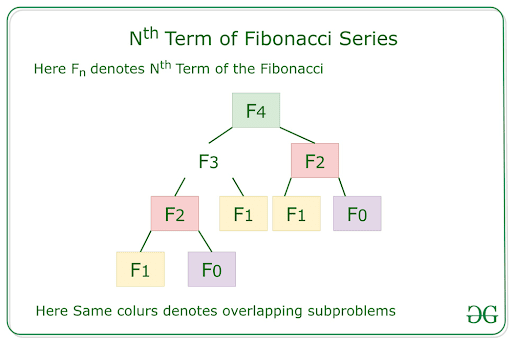
\includegraphics[height=5cm]{Pictures/ds-algo/nthfibonacciseriesdynamicprogramming.png}
        \end{figure}
    \end{minipage}
    \hfill
    \begin{minipage}{0.52\linewidth}
        \begin{itemize}
            \item \textbf{Subproblems}: $F(0)$, $F(1)$, $F(2)$, $F(3)$, ...
            \item \textbf{Store Solutions}: Create a table to store the values of $F(n)$ as they are calculated.
            \item \textbf{Build Up Solutions}: For $F(n)$, look up $F(n-1)$ and $F(n-2)$ in the table and add them.
            \item \textbf{Avoid Redundancy}: The table ensures that each subproblem (e.g., $F(2)$) is solved only once.
        \end{itemize}        
    \end{minipage}
\end{table}



\section{When to Use Dynamic Programming (DP)?}

\begin{enumerate}
    \item \textbf{Optimal Substructure}:\\
    Optimal substructure means that we combine the optimal results of subproblems to achieve the optimal result of the bigger problem.
    \item \textbf{Overlapping Subproblems}:\\
    The same subproblems are solved repeatedly in different parts of the problem.
\end{enumerate}

\section{Approaches of Dynamic Programming (DP)}

\subsection{Top-Down Approach (Memoization)}
In the top-down approach, also known as \textbf{memoization}, we start with the final solution and recursively break it down into smaller subproblems. To avoid redundant calculations, we store the results of solved subproblems in a memoization table. Suitable when the number of subproblems is large and many of them are reused.

\subsection{Bottom-Up Approach (Tabulation)}
In the bottom-up approach, also known as \textbf{tabulation}, we start with the smallest subproblems and gradually build up to the final solution. We store the results of solved subproblems in a table to avoid redundant calculations. Suitable when the number of subproblems is small and the optimal solution can be directly computed from the solutions to smaller subproblems.





























































































